\subsection{Analysis of Baselines}
% First, we will analyze the performance of the baseline models. Overall, the FC model is able to quickly gain performance at the start of training, but the performance saturates early on. The sub-optimal FC performance again demonstrates the need for complex models to capture temoral relationships among frames. Both the performance of MSTCN and DTGRM suffered from unbalanced verb class labels. DTGRM has shown better performance in segmenting short action instance. However, on long action instances, DTGRM does not perform as well as MSTCN as the predictions of DTGRM tends to be heavily over-segmented.

\paragraph{FC}
Since the classification is performed frame-wise and considers no temporal relations, the result is highly fragmental. We further note that the model tends to overfit at an early stage. The poor generalizability is indicated by the relatively low Edit score and Figure \ref{fig:baseline_qualitative}. %TODO: include graph. 


\paragraph{MSTCN} 
MSTCN demonstrates its effectiveness in segmenting out the most frequent label classes. 
We observe that the model assigns one of the most frequent verb classes when it struggles to label the action classes. The result implies that the model tends to memorize the label frequency.

To account for the complexity introduced by the large number of actions classes of EPIC-KITCHENS, we have tried 12-layer and 15-layer single-stage TCNs. We have also tried to increase the output channel size of the 1D convolutions from $64$ to $128$ or $256$. However, results from the experiments achieve similar performance as the ones for MS-TCN presented in Table \ref{table:results}; We believe that increasing number of layers and channels cannot improve the representation power of MS-TCN. 
\paragraph{DTGRM} 
Similar to MSTCN, DTGRM is able to output reasonable segmentation results. \ref{fig:baseline_qualitative} shows that one of its improvements from MSTCN is its capability in clearly segmenting out smaller segments, which proves the effectiveness of the additional fine-tuning component even on a more complex dataset like EPIC-KITCHENS. However, we also notice that DTGRM tend to over-segment on videos with fewer segments.

%DTGRM also suffers from the label class imbalance problem. Similar to MSTCN, it labels majority of the segments as the most frequent vocabulary classes in the training set. With the weighted loss, DTGRM is able to predict a wider variety of labels. However, the classification accuracy is not as high as in the original experiment \cite{wang2020temporal}. This is reasonable given the richer vocabulary classes available in EPIC-KITCHENS.

% Due to limitations on hardware, we are not able to expand the number of layers in the DTGRM model. To accommodate this, we sampled the feature inputs for every 10 frames of input to decrease input size. The more complex, sub-sampled DTGRM improved the over-segmentation issue in the original DTGRM by avoiding overly short segmentation under a sub-sampled setting.

%Dataset having unequal distribution of labels
%Learning the labels instead of learning the actual task
%Interesting point is that it learns backgrounds well, which could imply it knows "when" an action is taking place, just don't know "what" it is, so it guesses the most frequent action?%

\begin{figure*}[ht!]
\begin{center}
    \begin{minipage}[b]{1\textwidth}
        \begin{subfigure}[b]{0.475\textwidth}
            \centering
            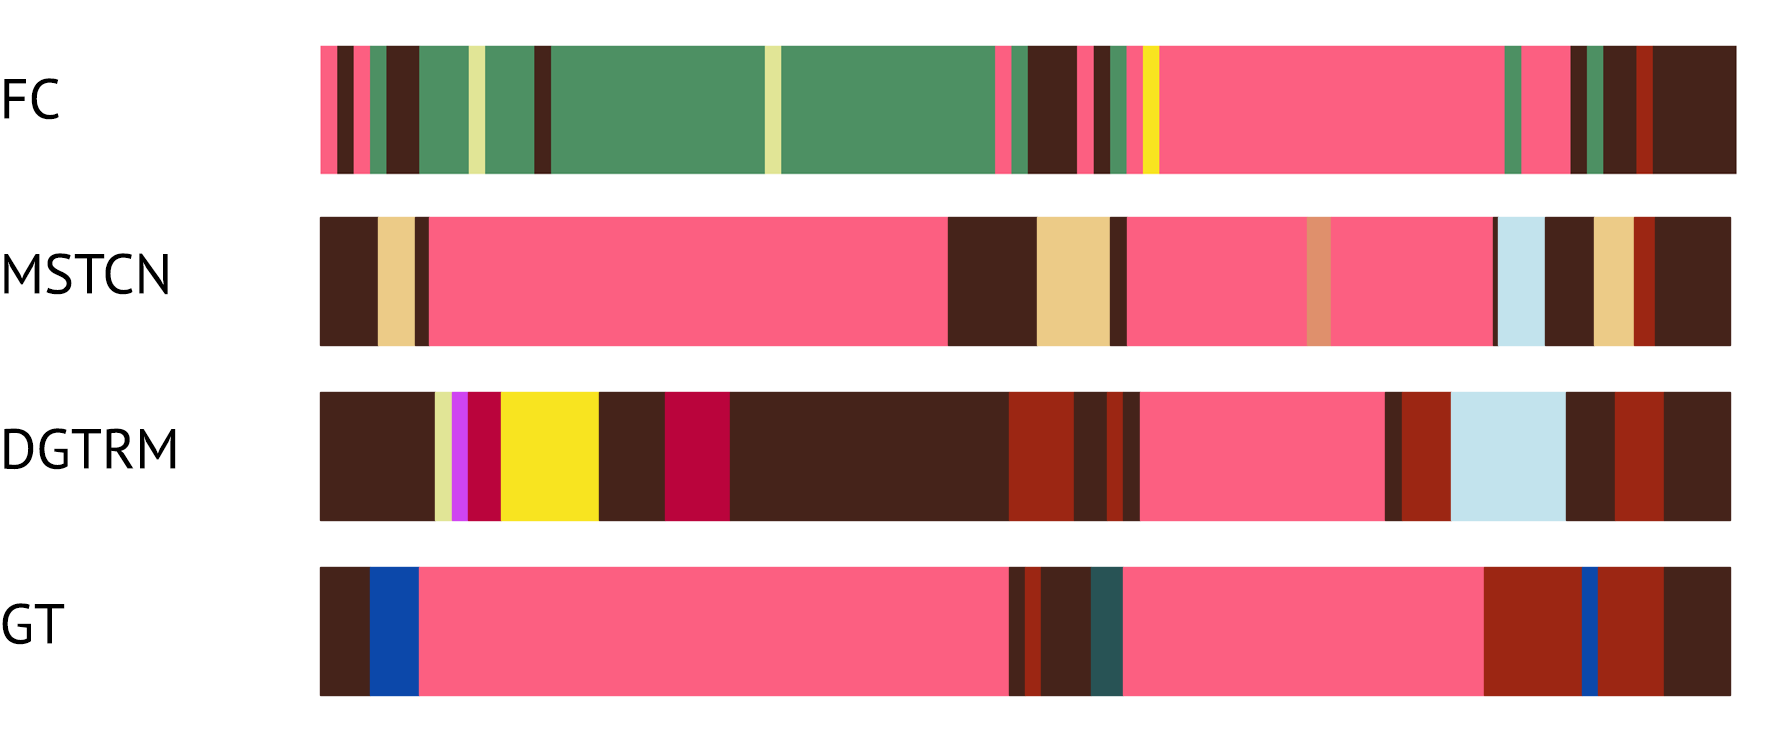
\includegraphics[scale=0.10]{figures/P26_39-comparison.png}
            \caption{Variation of Baseline Models}
            \label{fig:var_baseline}
        \end{subfigure}\quad
        \begin{subfigure}[b]{0.475\textwidth}
            \centering
            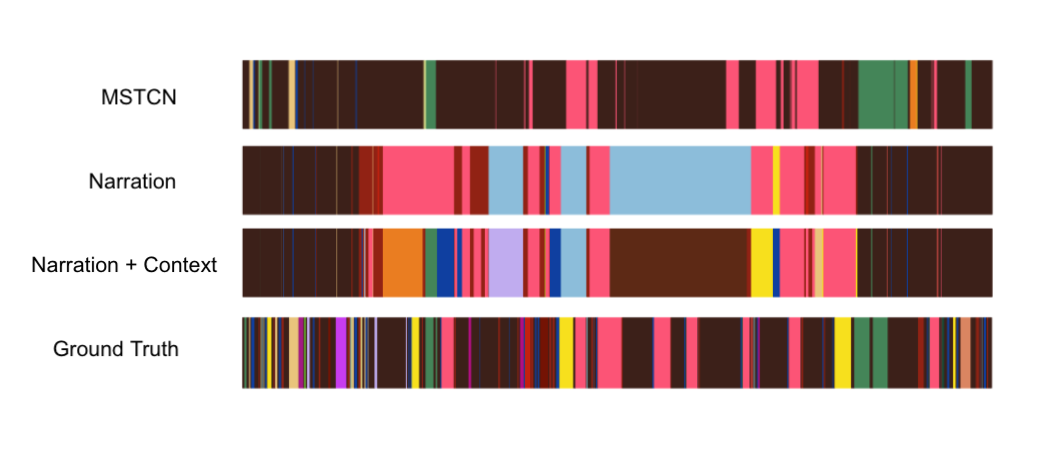
\includegraphics[scale=0.2]{figures/mstcn_howto100m.png}
            \caption{MS-TCN with Joint Embedding}
            \label{fig:mstcn_joint}
        \end{subfigure}
        \caption{Qualitative results of Methods}
        \label{fig:baseline_qualitative}
    \end{minipage}
\end{center}
\end{figure*}

%\paragraph{Loss function} 
%We experimented with two variants of loss function: cross-entropy loss with and without weighting. Since background frames comprise a sizable portion, one phenomenon we observe during training is that models tend to classify most of the frames as background, at least in the first few iterations. Down-weighting background classes can mitigate this issue, but inconsistency still exists between the loss function and metrics we used, since classifying frames as the most common verb class (e.g. background, \emph{wash}) can quickly increase frame-wise accuracy until some threshold (usually the percentage of these common verb class). From edit score, which reflects over-segmentation issue, we observe that models like MSTCN that incorporate temporal information tend to have higher Edit score than simpler models such as FC.  